\section{Auswertung}
\label{sec:Auswertung}

\subsection{Güteziffervergleich}
\begin{figure}
  \centering
  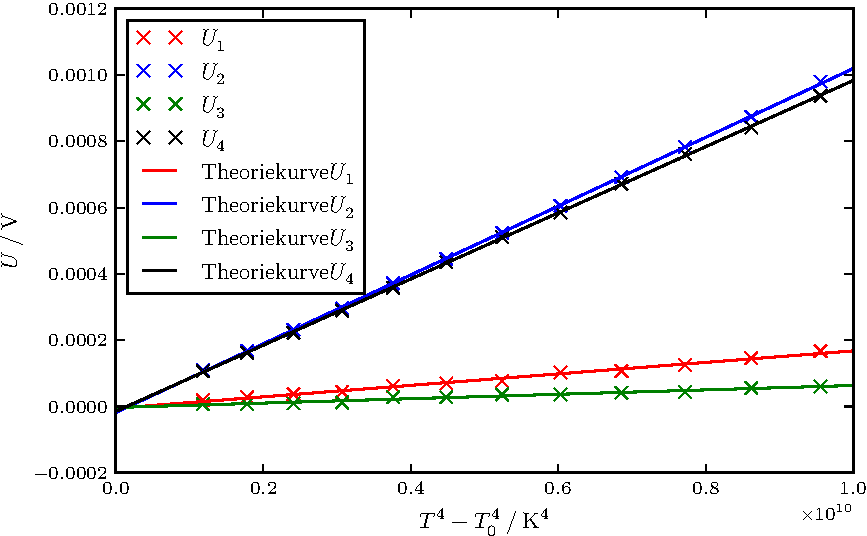
\includegraphics{plot.pdf}
  \caption{Plot.}
  \label{fig:plot}
\end{figure}
Die gemessenen Daten für die Tempeatur $T_1$ des wärmeren sowie die Temperatur
$T_2$ des kälteren Reservoirs wurden gegen die Zeit $t$ in Minuten abgetragen.
Mithilfe von SciPy wurde jeweils eine Ausgleichskurve für die folgende Funktion
berechnet:
\begin{equation}
  T(t)=A \cdot t^2 + B \cdot t + C
\end{equation}
Die Parameter $A$, $B$ und $C$ wurden bestimmt zu
\begin{align}
  A_{T_1} &= \SI{-0,01395 +- 0.00037}{\kelvin\per\minute²} & B_{T_1} &= \SI{1,40708 +- 0.01160}{\kelvin\per\minute} & C_{T_1} &= \SI{293,592 +- 0.075}{\kelvin} \\
  A_{T_2} &= \SI{0,01566 +- 0.00031}{\kelvin\per\minute²}  & B_{T_2} &= \SI{-1,08915 +- 0.00954}{\kelvin\per\minute} & C_{T_2} &= \SI{294,936 +- 0.062}{\kelvin}
\end{align}

Durch Ableiten und Einsetzen in die Ausgleichskurve
\begin{equation}
  \frac{\symup{d}T}{\symup{d}t}= 2 \cdot A \cdot t + B
\end{equation}
erhält man die Werte der Differentialquotienten. \\
Für eine ideale Wärmepumpe gilt
\begin{equation}
  v = \frac{T_1}{T_1-T_2}.
\end{equation}
Für die reale Wärmepunpe gilt jedoch die Formel
\begin{equation}
  v_{real}= \frac{\symup{d} Q_1}{\symup{d} tN} = (m_1c_w+m_kc_k)\frac{\symup{d} T_1}{\symup{d} tN}.
\end{equation}
Wobei $ N = $ der arithmetische Mittelwert der Kompressorleistung $ m_1 = ...$ die Masse des Wassers in $ R_1 $, $ c_w = ...$ die spezifische Wärmekapazität des Wassers und $ m_kc_k $ die Wärmekapazität der Kupferschlange und der Reservoire ist.
Die Werte sind in der Tabelle 1 aufgelistet.
\begin{equation}
\end{equation}

\subsection{Massendurchsatz}
